%%%%%%%%%%%%%%%%%%%%%%%%%%%%%%%%%%%%%%%%%
% Oliver Lemon made minor edits (jan 2015)  to : 
% Masters/Doctoral Thesis 
% LaTeX Template
% Version 1.43 (17/5/14)
%
% This template has been downloaded from:
% http://www.LaTeXTemplates.com
%
% Original authors:
% Steven Gunn 
% http://users.ecs.soton.ac.uk/srg/softwaretools/document/templates/
% and
% Sunil Patel
% http://www.sunilpatel.co.uk/thesis-template/
%
% License:
% CC BY-NC-SA 3.0 (http://creativecommons.org/licenses/by-nc-sa/3.0/)
%
% Note:
% Make sure to edit document variables in the Thesis.cls file
%
%%%%%%%%%%%%%%%%%%%%%%%%%%%%%%%%%%%%%%%%%

%----------------------------------------------------------------------------------------
%	PACKAGES AND OTHER DOCUMENT CONFIGURATIONS
%----------------------------------------------------------------------------------------

\documentclass[11pt, oneside]{Thesis} % The default font size and one-sided printing (no margin offsets)

\graphicspath{{Pictures/}} % Specifies the directory where pictures are stored

\usepackage[square, comma, sort&compress]{natbib} % Use the natbib reference package - read up on this to edit the reference style; if you want text (e.g. Smith et al., 2012) for the in-text references (instead of numbers), remove 'numbers' 
\hypersetup{urlcolor=blue, colorlinks=true} % Colors hyperlinks in blue - change to black if annoying


\title{UoE CS Masters thesis template} % BUT you should use use " \title{\ttitle} " here instead to define the thesis title ! 
% \ttitle is defined in the file Thesis.cls 

\begin{document}

\frontmatter % Use roman page numbering style (i, ii, iii, iv...) for the pre-content pages

\setstretch{1.3} % Line spacing of 1.3

% Define the page headers using the FancyHdr package and set up for one-sided printing
\fancyhead{} % Clears all page headers and footers
\rhead{\thepage} % Sets the right side header to show the page number
\lhead{} % Clears the left side page header

\pagestyle{fancy} % Finally, use the "fancy" page style to implement the FancyHdr headers

\newcommand{\HRule}{\rule{\linewidth}{0.5mm}} % New command to make the lines in the title page

% PDF meta-data
\hypersetup{pdftitle={\ttitle}}
\hypersetup{pdfsubject=\subjectname}
\hypersetup{pdfauthor=\authornames}
\hypersetup{pdfkeywords=\keywordnames}

%----------------------------------------------------------------------------------------
%	TITLE PAGE
%----------------------------------------------------------------------------------------

\begin{titlepage}
\begin{center}

\textsc{\LARGE \univname}\\[1.5cm] % University name
\textsc{\Large Masters Thesis}\\[0.5cm] % Thesis type

\HRule \\[0.4cm] % Horizontal line
{\huge \bfseries \ttitle}\\[0.4cm] % Thesis title
\HRule \\[1.5cm] % Horizontal line
 
\begin{minipage}{0.4\textwidth}
\begin{flushleft} \large
\emph{Author:}\\
\href{}{\authornames} % Author name - remove the \href bracket to remove the link
\end{flushleft}
\end{minipage}
\begin{minipage}{0.4\textwidth}
\begin{flushright} \large
\emph{Supervisors:} \\
\href{}{\supname} % Supervisor name - remove the \href bracket to remove the link  
\end{flushright}
\end{minipage}\\[3cm]
 
\large \textit{A thesis submitted in fulfilment of the requirements\\ for the degree of \degreename}\\[0.3cm] % University requirement text
\textit{in the}\\[0.4cm]
%\groupname\\

\deptname\\[2cm] % Research group name and department name
 
{\large \today}\\[1cm] % Date

\includegraphics[width=6cm]{./Figures/UoE_logo.png} % University/department logo - uncomment to place it
 
\vfill
\end{center}

\end{titlepage}

%----------------------------------------------------------------------------------------
%	DECLARATION PAGE
%	Your institution may give you a different text to place here
%----------------------------------------------------------------------------------------

\Declaration{

\addtocontents{toc}{\vspace{1em}} % Add a gap in the Contents, for aesthetics

I, \authornames, declare that this thesis titled, '\ttitle' and the work presented in it is my own. I confirm that this work submitted for assessment is my own and is
  expressed in my own words. Any uses made within it of the works of
  other authors in any form (e.g., ideas, equations, figures, text,
  tables, programs) are properly acknowledged at any point of their
  use. A list of the references employed is included.

%\begin{itemize} 
%\item[\tiny{$\blacksquare$}] This work was done wholly or mainly while in candidature for a research degree at this University.
%\item[\tiny{$\blacksquare$}] Where any part of this thesis has previously been submitted for a degree or any other qualification at %this University or any other institution, this has been clearly stated.
%\item[\tiny{$\blacksquare$}] Where I have consulted the published work of others, this is always clearly attributed.
%\item[\tiny{$\blacksquare$}] Where I have quoted from the work of others, the source is always given. With the exception of such %quotations, this thesis is entirely my own work.
%\item[\tiny{$\blacksquare$}] I have acknowledged all main sources of help.
%\item[\tiny{$\blacksquare$}] Where the thesis is based on work done by myself jointly with others, I have made clear exactly what %was done by others and what I have contributed myself.\\
%\end{itemize}
 \vspace{2cm} 
Signed:\\
\rule[1em]{25em}{0.5pt} % This prints a line for the signature
 
Date:\\
\rule[1em]{25em}{0.5pt} % This prints a line to write the date
}

\clearpage % Start a new page
% * <anse23@hotmail.com> 2018-06-18T10:13:39.223Z:
%
% ^.
% * <anse23@hotmail.com> 2018-06-18T10:13:36.948Z:
%
% ^.

%----------------------------------------------------------------------------------------
%	QUOTATION PAGE
%----------------------------------------------------------------------------------------

\pagestyle{empty} % No headers or footers for the following pages

\null\vfill % Add some space to move the quote down the page a bit

\textit{``Thanks to my solid academic training, today I can write hundreds of words on virtually any topic without possessing a shred of information, which is how I got a good job in journalism."}

\begin{flushright}
Dave Barry
\end{flushright}

\vfill\vfill\vfill\vfill\vfill\vfill\null % Add some space at the bottom to position the quote just right

\clearpage % Start a new page

%----------------------------------------------------------------------------------------
%	ABSTRACT PAGE
%----------------------------------------------------------------------------------------

\addtotoc{Abstract} % Add the "Abstract" page entry to the Contents

%\abstract{\addtocontents{toc}{\vspace{1em}} % Add a gap in the Contents, for aesthetics

 {\huge{\textit{Abstract}} \par}{\addtocontents{toc}{\vspace{1em}} 

The Thesis Abstract is written here (and usually kept to just this page). 
%The page is kept centered vertically so can expand into the blank space above the title too\ldots
%

\clearpage % Start a new page

%----------------------------------------------------------------------------------------
%	ACKNOWLEDGEMENTS
%----------------------------------------------------------------------------------------

\setstretch{1.3} % Reset the line-spacing to 1.3 for body text (if it has changed)

\acknowledgements{\addtocontents{toc}{\vspace{1em}} % Add a gap in the Contents, for aesthetics

The acknowledgements and the people to thank go here, don't forget to include your project advisor :)  
}
\clearpage % Start a new page

%----------------------------------------------------------------------------------------
%	LIST OF CONTENTS/FIGURES/TABLES PAGES
%----------------------------------------------------------------------------------------

\pagestyle{fancy} % The page style headers have been "empty" all this time, now use the "fancy" headers as defined before to bring them back

\lhead{\emph{Contents}} % Set the left side page header to "Contents"
\tableofcontents % Write out the Table of Contents

\lhead{\emph{List of Figures}} % Set the left side page header to "List of Figures"
\listoffigures % Write out the List of Figures

\lhead{\emph{List of Tables}} % Set the left side page header to "List of Tables"
\listoftables % Write out the List of Tables

%----------------------------------------------------------------------------------------
%	ABBREVIATIONS
%----------------------------------------------------------------------------------------

\clearpage % Start a new page

\setstretch{1.5} % Set the line spacing to 1.5, this makes the following tables easier to read

\lhead{\emph{Abbreviations}} % Set the left side page header to "Abbreviations"
\listofsymbols{ll} % Include a list of Abbreviations (a table of two columns)
{
\textbf{LAH} & \textbf{L}ist \textbf{A}bbreviations \textbf{H}ere \\
%\textbf{Acronym} & \textbf{W}hat (it) \textbf{S}tands \textbf{F}or \\
}

%----------------------------------------------------------------------------------------
%	PHYSICAL CONSTANTS/OTHER DEFINITIONS
%----------------------------------------------------------------------------------------

%\clearpage % Start a new page

%\lhead{\emph{Physical Constants}} % Set the left side page header to "Physical Constants"

%\listofconstants{lrcl} % Include a list of Physical Constants (a four column table)
%{
%Speed of Light & $c$ & $=$ & $2.997\ 924\ 58\times10^{8}\ \mbox{ms}^{-\mbox{s}}$ (exact)\\

%% Constant Name & Symbol & = & Constant Value (with units) \\
%}

%----------------------------------------------------------------------------------------
%	SYMBOLS
%----------------------------------------------------------------------------------------

\clearpage % Start a new page

\lhead{\emph{Symbols}} % Set the left side page header to "Symbols"

\listofnomenclature{lll} % Include a list of Symbols (a three column table)
{
$a$ & distance & m \\
$P$ & power & W (Js$^{-1}$) \\
% Symbol & Name & Unit \\

& & \\ % Gap to separate the Roman symbols from the Greek

$\omega$ & angular frequency & rads$^{-1}$ \\
% Symbol & Name & Unit \\
}

%----------------------------------------------------------------------------------------
%	DEDICATION
%----------------------------------------------------------------------------------------

\setstretch{1.3} % Return the line spacing back to 1.3

\pagestyle{empty} % Page style needs to be empty for this page

\dedicatory{For/Dedicated to/To my\ldots} % Dedication text

\addtocontents{toc}{\vspace{2em}} % Add a gap in the Contents, for aesthetics

%----------------------------------------------------------------------------------------
%	THESIS CONTENT - CHAPTERS
%----------------------------------------------------------------------------------------

\mainmatter % Begin numeric (1,2,3...) page numbering

\pagestyle{fancy} % Return the page headers back to the "fancy" style

% Include the chapters of the thesis as separate files from the Chapters folder
% Uncomment the lines as you write the chapters

% Chapter 1

\chapter{Introduction} % Main chapter title

\label{intro} % For referencing the chapter elsewhere, use \ref{Chapter1} 

\lhead{Chapter 1. \emph{Introduction}} % This is for the header on each page - perhaps a shortened title

%----------------------------------------------------------------------------------------
\section{Gamification}
Gamification can be defined as the process of adding game elements and mechanics in non-game contexts \citep{deterding2011game}. The main objective of Gamification is to improve the user's experience and increase the motivation to use a product or service. To accomplish such objective, Gamification takes advantage of the inherent nature of humans to play. Unlike mandatory activities such study and work, play is voluntary and free; its main outcome is a feeling of joy and excitement \citep{johan1950homo}. These conditions set the environment for the adoption of game concepts and techniques in broader contexts.

Over the past ten years, Gamification has attracted the attention of industry and academia. In the industry, companies have found a means to improve the performance and commitment of employees by avoiding traditional schemes of monetary rewards and punishments. Morevover, Gamification provides a set of tools to increase the loyalty and engagement of users and customers. For the academia, Gamification has expanded and merged various field of research given its interdisciplinary nature. It has attracted the attention of researchers in areas such as Human Computer Interaction, Software Development, Psychology, Pedagogy, Bussiness Management and others.

%----------------------------------------------------------------------------------------
\section{Spaced Repetition}
Spaced Repetition is a technique that facilitates the retention of new knowledge. It leverages the spacing effect phenomenon to help learners memorize specific contents \citep{hintzman1974theoretical}. This phenomenon allows learners to increase their capacity of retention by acquiring new knowledge in short recurrent sessions rather than in a single massive revision. In its basic form, Spaced Repetition sets increasing intervals of time between subsequent review sessioins of previously learned material. This means that the more challenging the content, the more frequently is reviewed by a learner. Then, the frequency of repetition is adjusted as the learner progresses.

Among the various existing techniques for memorization, Spaced Repetition stands out due to its simplicity and flexibility. The duration of each revision along with the inteval time between consecutive sessions is defined by the learner. In addition, the learner assesses the easiness of the content under revision to determine the frequency of repetition. Finally, Spaced Repetition is a technique that can be used to learn new content from any field, but it is specially useful when the number of items to memorize is large. Such characteristics allow the implementation of this technique as a piece of software, making it available to a wider audience.

%----------------------------------------------------------------------------------------
\section{Motivation}
Activities such as using a tool, executing an action, or adopting a behaviour have an underlying incentive. In many cases, such incentive is the obtaining of a reward in the form of a monetary compensation for a job, or good marks in a study program. The lack of additional incentive factors can make people stop doing such activities once the reward is obtained. Likewise, activities that do not offer specific rewards but provide other benefits are also affected by the absence of extra incentive elements. In contrast, activities that people do for joy or entertainment are likely to be repeated over time. 

In the specific case of Spaced Repetition, the main incentive to use it is the memorization of new content. However, its flexibility to let users define the duration of each session and the interval between consecutive revisions can lead to a gradual reduction of its usage over time. Such circumstance avoids the learners to keep getting the benefits of the technique. These conditions set a perfect environment for the adoption of a gamification scheme that provides new incetives to the learners. This way users of Spaced Repetition can mantain a constant pace of study while enjoying the experience.
%---------------------------------------------------------------------------------------
%% Chapter 1

\chapter{Background} % Main chapter title

\label{back} % For referencing the chapter elsewhere, use \ref{Chapter1}

\lhead{Chapter 2. \emph{
Background}} % This is for the header on each page - perhaps a shortened title
The present work relied on two important concepts: gamification and spaced repetition. An overview of both concepts sets the stage for the proposed solution. Gamification provides an alternative to improve user experience, whereas spaced repetition offers a way to ease the retention of new knowledge. Among the several alternatives that implement spaced repetition, Anki and its mobile interface, AnkiDroid, provide a general purpose approach with a large user base. In addition, casual games offer characteristics that make them adaptable to non-leisure contexts including learning. One example is the 2048 game \citep{uberspot2017game} that has been subject of several studies. Finally, statistical testings allow to make inferences about the outcome of an experiment.

%----------------------------------------------------------------------------------------
\section{Gamification}
Gamification can be defined as the process of adding game elements and schemes into non-game contexts \citep{deterding2011game}. The main objective of gamification is to improve the user experience and increase the motivation to use a product or service. To accomplish such an objective, gamification takes advantage of the inherent nature of humans to play. Unlike mandatory activities such as study and work, playing is voluntary and free; its main outcome is a feeling of joy and excitement \citep{johan1950homo}. These conditions set the environment for the adoption of game concepts and techniques in broader contexts.

Over the past ten years, gamification has attracted the attention of industry and academia. In the industry, companies have found a means to improve the performance and commitment of employees by avoiding traditional schemes of monetary rewards and punishments. Moreover, gamification provides a set of tools to increase the loyalty and engagement of users and customers. In the academia, gamification has expanded and merged various field of research given its interdisciplinary nature. It has attracted the attention of researchers in areas such as Human-Computer Interaction, Software Development, Psychology, Pedagogy, Bussiness Management and others.

Among the many concepts related to gamification, there are three that need to be clearly identified to set the bases of a gamification strategy. The first one is game element which refers to the specific pieces taken from games, such as points, rewards, achievements, etc. The second one is game scheme or game mechanics which refers to the rules that users need to follow to get a certain outcome. Finally, a player is the person that uses the gamified system.

%----------------------------------------------------------------------------------------
\section{Spaced Repetition}
Spaced repetition is a technique that facilitates the retention of new knowledge. It leverages the spacing effect phenomenon to help learners memorize specific contents \citep{hintzman1974theoretical}. This phenomenon allows learners to increase their capacity of retention by acquiring new knowledge in short recurrent sessions rather than in a single massive revision. In its basic form, spaced repetition sets increasing intervals of time between subsequent review sessions of previously learned material. This means that the more challenging the content the more frequently is reviewed by a learner. Then, the frequency of repetition is adjusted as the learner progresses.

Among the various existing techniques for memorization, spaced repetition stands out due to its simplicity and flexibility. The duration of each revision along with the interval time between consecutive sessions is defined by the learner. In addition, the learner assesses the easiness of the content under revision to determine the frequency of repetition. Finally, Spaced Repetition is a technique that can be used to learn new content from any field, but it is especially useful when the number of items to memorize is large. Such characteristics allow the implementation of this technique as a piece of software, making it available to a wider audience.

%----------------------------------------------------------------------------------------
\section{AnkiDroid}
Anki is a platform that implements a general purpose solution for spaced repetition. Thus, it can be used to learn and memorize content from any field. Its community has created an extensive base of content in a multitude of categories including languages, art, science, and trivia. It provides several interfaces including desktop applications for Linux, Mac, and Windows. In mobile environments, it provides applications for iOS and Android devices. The version for Android devices is known as AnkiDroid which code is publicly available under the GNU general public license.

AnkiDroid has well-defined logic and visual structures \citep{zamora2011ankidroid} that implement most of the features presented in the desktop applications including creation and editing of flashcards, visualization of statistics of use, and synchronization with the Anki system to save progress. Moreover, it has been designed to be compatible with the majority of Android versions. Therefore, the application is available for a wide range of devices which have helped to increase its popularity as an educational tool as seen in Figure \ref{fig:anki-evolution}.

In addtion, AnkiDroid has an large community of members that collaborate, support and promote the use and development of the application in web forums and groups. In regards to its development, the structure of the code allows modifications in the application that add or remove new features. The application can be modified to connect to external services, collect information of use, or include new elements. These characteristics have allowed that an extensive number of contributors (131) be part of its development.

\begin{figure}[htb]
    \vskip 5mm
        \begin{center}
            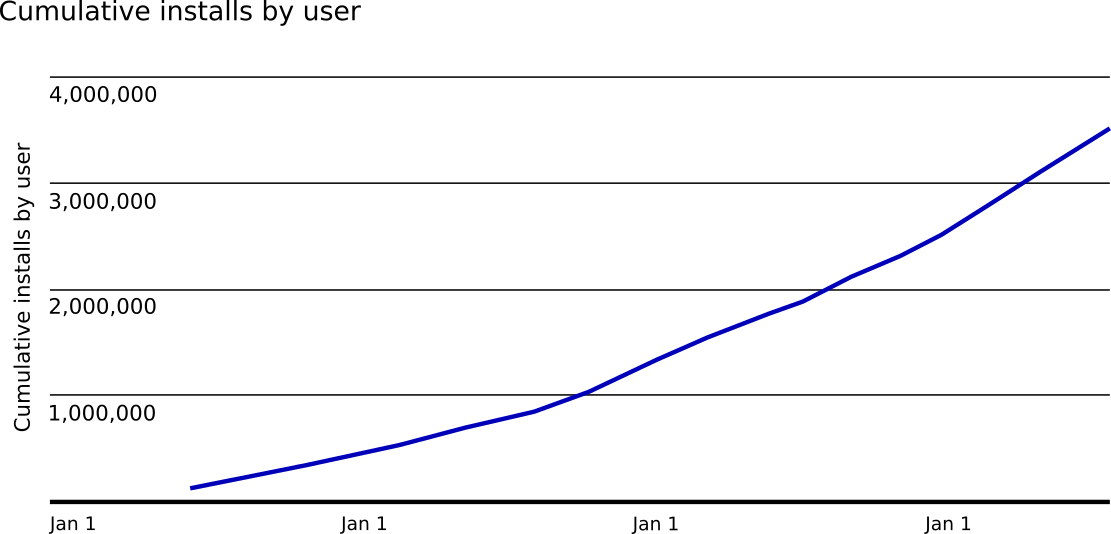
\includegraphics[scale=0.4]{./Figures/anki_progress.png}
            \caption{Evolution of the number of installations of AnkiDroid. Image taken from the twitter account of AnkiDroid (https://twitter.com/AnkiDroid)}
            \label{fig:anki-evolution}
        \end{center}
    \vskip -5mm
\end{figure}


%----------------------------------------------------------------------------------------
\section{Casual Video Games}
A casual game has to be fun, it needs to provide a quick way to access, and the gameplay must be easy to understand, as defined by the Casual Games Association (CGA). These characteristics mean that users do not require any previous expertise or skills related to video games. For these reasons, casual games have a broad audience that includes people from all age groups.

The characteristics of this type of games have been leverage to adapt them to non-leisure contexts including health and learning. In the health context, the use of casual games has been studied as an alternative element to improve mood and decrease stress \citep{russoniello2009effectiveness}. Additional studies have demonstrated the effectiveness of playing casual games as a recovery strategy after periods of high work strain \citep{reinecke2009games}. Finally, casual games have also been studied as an alternative to traditional educational tools \citep{peirce2010personalised}

%----------------------------------------------------------------------------------------
\section{2048 Game}
2048 is a puzzle-like casual game cotaining a 4x4 grid as seen in Figure \ref{fig:2048-grid}. The objective of the game is to merge numbered blocks until creating one with the value 2048. The game starts with two blocks of value 2 which are randomly positioned in the grid. The player has to slide the blocks horizontally or vertically. The blocks move in the chosen direction; a block stops if it reaches an edge of the grid or collides with another block. If two colliding blocks have the same number, they are merged into a single block which value is the sum of the values of the forming blocks. In every turn, a new block of value 2 is randomly positioned in the grid.

\begin{figure}[htb]
    \vskip 5mm
        \begin{center}
            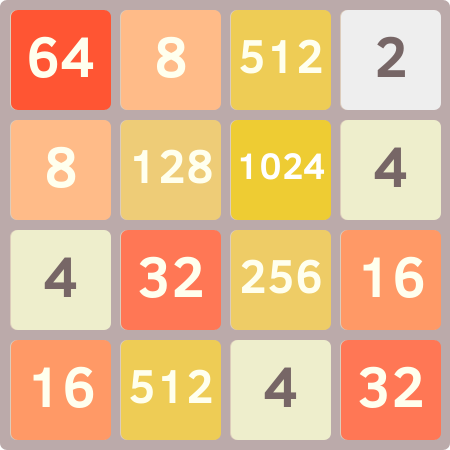
\includegraphics[scale=0.5]{./Figures/game_grid.png}
            \caption{Grid of the 2048 game.}
            \label{fig:2048-grid}
        \end{center}
    \vskip -5mm
\end{figure}

The popularity of the game has turned it into a subject of different types of studies. The majority of these studies aim to analyse the game from the computational complexity perspective \citep{abdelkader20162048}, and propose several artificial intelligence alternatives to win the game including neural networks \citep{boris2016evolving} and Monte-Carlo methods \citep{rodgers2014investigation}. However, the game has also been studied as an educational element to engage student interest \citep{neller2015pedagogical}

%----------------------------------------------------------------------------------------
\section{Statistical testing}
\label{stat-testing}
Statistical testing provides a way to make inferences about the data and tell if the observed pattern is real or due to chance. In research, this type of analysis helps to determine the effects of a treatment on the outcome and the robustness of that relationship. In comparative studies, a new treatment is applied to units in the experimental group, whereas units in the control group receive the standard treatment or not treatment at all.

The outcomes from the control and experimental groups can be described and compared by their means. The difference between both means gives some insights about the groups. However, the difference of means needs to be complimented with the variances of the samples to determine if it is statistically significant. This analysis can be done using the Student's t-test.

The Student's t-test is a method that can be used to do a statistical hyphotesis testing. The method provides a parameter called \textit{t-value} that is the ratio bewteen a signal (difference of means) and noise (variability of samples). This parameter and the degrees of freedom (number of values that are free to vary) are used to find the \textit{p-value} which is probability value of having the same mean difference in additional experiments. Therefore, the \textit{p-value} is used to confirm or deny the null hypothesis of the experiment.

% % Add to description of game
%  the state of the grid is defined by the positions of the blocks and their values at a given turn
 
%% Chapter 1

\chapter{Related Work} % Main chapter title

\label{rela} % For referencing the chapter elsewhere, use \ref{Chapter1} 

\lhead{Chapter 3. \emph{Related Work}} % This is for the header on each page - perhaps a shortened title

%----------------------------------------------------------------------------------------
\section{Learning and Gamification}

%----------------------------------------------------------------------------------------
\section{Previous attempts to gamify AnkiDroid}

%% Chapter 4

\chapter{Design and Implementation} % Main chapter title

\label{desi} % For referencing the chapter elsewhere, use \ref{desi}

% \lhead{Chapter 4. \emph{Design and Implementation}} % This is for the header on each page - perhaps a shortened title
The inclusion of game schemes and elements in AnkiDroid required an analysis of its original design. The purpose was finding suitable parts in the structure of the application to integrate gamification components. Once these parts were found, the next step was to set an initial gamification strategy to modify the application. Later, it was necessary to design an approach to include a casual game. Such an approach needed to define a scheme to link the game to reviewing flashcards by means of the initial gamification strategy as seen in Figure \ref{fig:game-elem-cards}. Finally, it was necessary to consider user interface aspects for a smooth integration of the overall solution.

\begin{figure}[htb]
    \vskip 5mm
        \begin{center}
            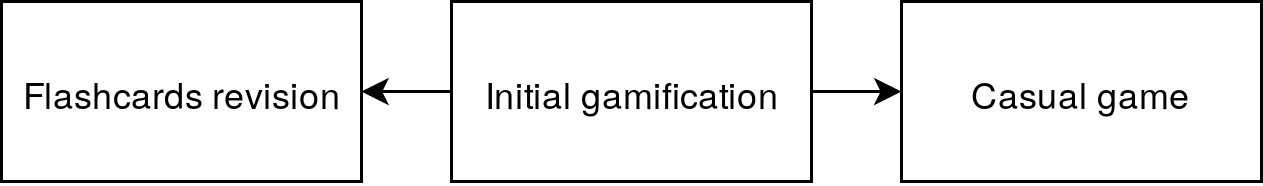
\includegraphics[scale=0.3]{./Figures/design.png}
            \caption{High level view of the design components and their relationships.}
            \label{fig:game-elem-cards}
        \end{center}
    \vskip -5mm
\end{figure}


%----------------------------------------------------------------------------------------
\section{Components of Interest in AnkiDroid}
\label{desi-components-interest}
AnkiDroid is a mature application with a clear structure and well-defined logic. It has a user interface that follows the best design principles for mobile development. Despite its multiple features and functionalities, the core element is the flashcard reviewer. Here is where the application allows the users to benefit from the effects of spaced repetition. The available interactions to review flashcards permit the user to progress by checking the front of a flashcard (question), revealing its back (answer), and assessing it, which automatically leads to a new flashcard as seen in Figure \ref{fig:front-back-assess}.

\begin{figure}[htb]
    \vskip 5mm
        \begin{center}
            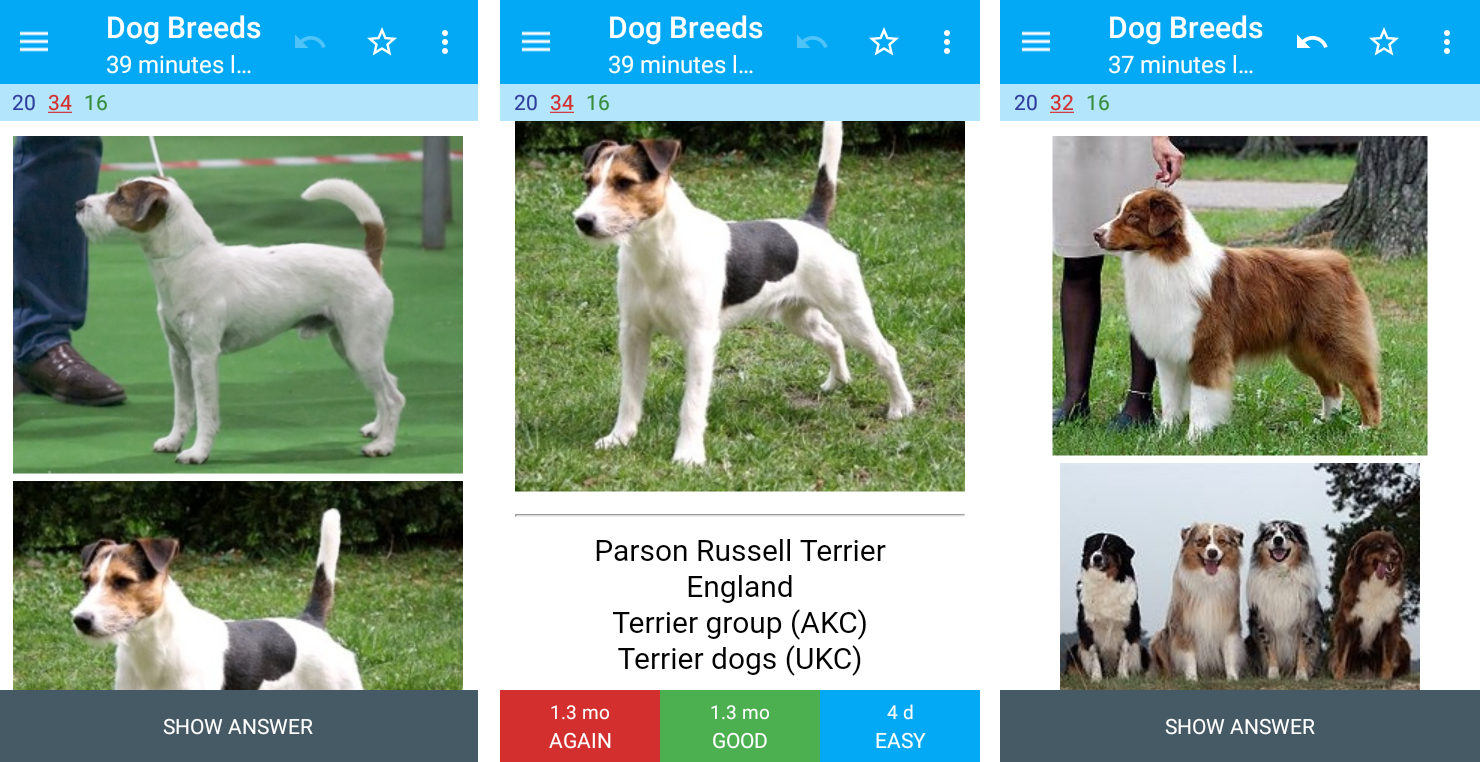
\includegraphics[scale=0.28]{./Figures/reviewer.png}
            \caption{Flashcard reviewer showing the front, back, front flow.}
            \label{fig:front-back-assess}
        \end{center}
    \vskip -5mm
\end{figure}

Many other secondary components are developed around the revision of flashcards, with the deck picker as the most relevant one. This component is the first contact users have with the application. Its main role is displaying the available decks of flashcards as seen in Figure \ref{fig:deck-picker}. It also allows several actions on the decks including selection, deletion, and addition. When users select a deck, the application starts the flashcards revision process. The deck picker connects to other parts of the application like statistics and settings. Finally, the deck picker displays other information including the number of flashcards and the time reviewing them.

\begin{figure}[htb]
    \vskip 5mm
        \begin{center}
            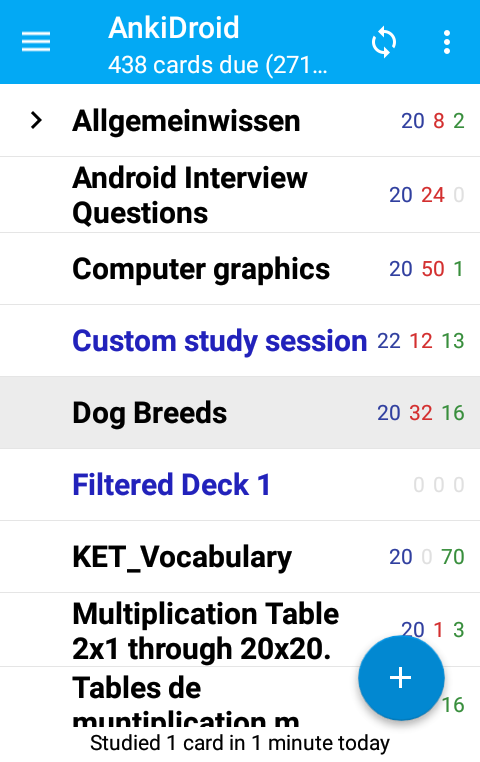
\includegraphics[scale=0.4]{./Figures/picker.png}
            \caption{Deck picker showing the decks of flashcards.}
            \label{fig:deck-picker}
        \end{center}
    \vskip -5mm
\end{figure}

The visual and logic characteristics of the flashcard reviewer and the deck picker were used to facilitate the inclusion of game elements and schemes. Visually, both elements present a structure that allows a smooth incorporation of new elements that do not interfere with their main purpose. In regard to logic, the deck picker allows getting access to new components of the application. On the other hand, the flashcard reviewer has a flow of events that can be linked to additional actions, which could provide instant feedback to users.

%----------------------------------------------------------------------------------------
\section{Initial Gamification Strategy}
\label{desi-gamification-strategy}
The process started with the definition of a model of extrinsic motivation based on rewards \citep{richter2015studying}. The basic tangible component of this model had the form of points, which were tied to the revision of flashcards. The approach was extended to include coins as an additional reward element that complemented the role of points. Points and coins presented characteristics that allowed them to be used beyond the reward model. However, coins differed from points on how they could vary in number and the way users could use them.

The model of motivation was extended to include more advanced game elements built upon the basic rewards. It incorporated a set of achievements that was defined based on the number of points. The achievements were also set to provide a more game-like mood to the overall user experience. Later, a customisation scheme made use of the characteristics of points to link them to achievements. Points along with customisation were also used to define a social and competition scheme. Additional elements were defined to keep users informed about their progress.

%----------------------------------------------------------------------------------------
\subsection{Rewards}
In games, a reward is something given to a player as the result of executing a task. In many cases, the objective is to motivate the player to do the same task again. In addition, rewards can also be defined as resources for later use; therefore, they can be accumulated. Based on this scheme, a virtual currency was defined in the form of coins. Since the core of the application was the revision of flashcards, such coins were given to users each time a flashcard was reviewed. Specifically, the number of available coins was increased each time the user assessed a flashcard.

A reward scheme requires the benefit the player receives to be proportional to the effort done. The content of the flashcards varied from one deck to another; it could be as simple as text, or as complex as images and audio. Therefore, the effort exerted in each flashcard was different. Thus, the number of coins granted in each flashcard was defined by the amount of effort. The most suitable way to calculate the effort of users based on the content of flashcards was by measuring the time spent on them. Hence, the number of coins per flashcard was defined as a function of time. However, a couple of restrictions had to be considered to avoid undesired behaviours from users.

Given that coins were also resources, users could be tempted to obtain them with minimal effort. One potential misbehaviour was passing flashcards as fast as possible to obtain the highest number of possible coins. Moreover, users could intentionally spend more time reviewing flashcards to obtain more coins. Diminishing these issues required setting ranges of time. Therefore, there were three ranges to calculate the number of coins in each flashcard: null, linear, and constant. The null range was one second long and started the moment a question or an answer was displayed. The linear range was three seconds long, and the number of coins was proportional to the amount of time. Finally, the constant range lasted until a new answer or question was displayed and no coins were given.

\begin{equation}
  c(t) =
      \begin{cases}
        0 & \text{if t $\leq$ 1}\\
        t & \text{if 1 $<$ t $\leq$ 3}\\
        3 & \text{if t $>$ 3}\\
      \end{cases}
    \label{eq:coins-formula}
\end{equation}

Equation \ref{eq:coins-formula} describes the calculation of coins, where \textit{c} is the number of coins as a function of the elapsed time in seconds, \textit{t}. The number of coins was always an integer value. It is important to note that there were minimum and maximum numbers of coins that could be earned in each flashcard, 0 and 6 (3 for the question and 3 for the answer) respectively. A potential drawback when calculating coins was the repetition of a flashcard since AnkiDroid allows undoing the previously reviewed flashcard. Therefore, users could earn additional coins for the same flashcard. However, reviewing a previous flashcard again was not penalised, and the previously earned coins were kept.

Coins could be spent by users to get benefits that will be explained later. This dynamic characteristic and how they were calculated could potentially reduce their potential benefits as rewards. Thus, it was necessary to implement a new element with a similar earning scheme but additional characteristics. Points are common elements in games. Their objective varies from context to context, but usually, they are used as additional rewards and provide information about progress since they are accumulative. Other educational platforms have added points as a motivational element \citep{disalvo2014khan}.

Points were designed to be calculated in a similar way to coins. There existed ranges of time to earn coins. The first range had the same objective as the one for coins, so, its duration was similar. A second range was meant to earn coins proportionally to the time; however, the relation is not linear but logarithmic as seen in Equation \ref{eq:points-formula}, where \textit{p} is the number of points as a function of the elapsed time in seconds, \textit{t}. Since logarithms are negative for values less than one, a max function between 1 and the logarithm was applied to avoid negative points. Finally, the number of coins was always an integer.

The logarithmic relation and the lack of a limit for points had two objectives. First, the creation of an additional distinction between points and coins. If the number of coins and points in a flashcard were greater than 0, it was unlikely that they were the same value. The second goal had to do with the limit for coins. Since the content of some flashcards could require more time than usual to review, the maximum number of coins per flashcard acted as a penalisation for flashcards with large content. Therefore, the lack of a limit for the number of points earned in a flashcard compensated for the coins penalisation in large flashcards.

\begin{equation}
  p(t) =
      \begin{cases}
        0 & \text{if t $\leq$ 1}\\
        max(1, 10log(t)) & \text{if t $>$ 1}\\
      \end{cases}
    \label{eq:points-formula}
\end{equation}

%----------------------------------------------------------------------------------------
\subsection{Achievements}
Rewards are by nature obtained after doing small tasks. Several games implement more advanced elements that increase the players' motivation; they are known as achievements. They are similar to rewards, but the main difference is the size of the tasks to get them. Those tasks usually require more time, the execution of a sequence of steps, or the repetition of smaller tasks. The most basic task in AnkiDroid is the revision of flashcards, which served to define the achievements scheme; moreover, the accumulative nature of points was also useful in the design.

In the solution, the achievements were designed to be obtained after the repetition of a small task (revision of flashcards). The number of points was used as the element to inform users of the progress to reach each achievement. Unlike rewards like coins or points that do not have a limit, achievements were defined as a set of specific elements to be gotten with a specific number of points. Therefore, users were aware of the number of available achievements and the required points to obtain them. Moreover, the application provided information about the reached achievements and the remaining ones.

In addition, to give AnkiDroid a more game-like mood, achievements were depicted as pets to be rescued. Those pets were called ankimals, a term that merges the words Anki and animals to provide a sense of identity with the application. The feeling of rescuing pets was complemented with notifications to inform users when a new ankimal was freed. The notifications were designed to encourage the users to rescue more pets by earning more points; therefore, they indirectly asked users to review more flashcards as seen in Figure \ref{fig:ankimals-rescue}.

\begin{figure}[htb]
    \vskip 5mm
        \begin{center}
            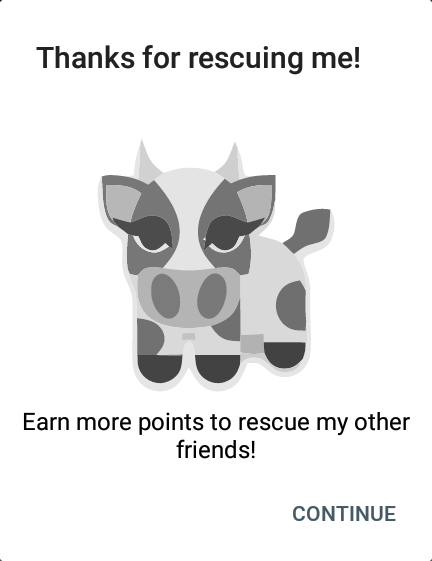
\includegraphics[scale=0.35]{./Figures/achievement_notification.png}
            \caption{Notification shown to user when achievement is reached.}
            \label{fig:ankimals-rescue}
        \end{center}
    \vskip -5mm
\end{figure}

%----------------------------------------------------------------------------------------
\subsection{Customisation}
Games provide customization aspects to give a more personal experience to players. In the solution, this scheme was defined with two elements. The first one was a nickname that could be set by the user. This element was meant to give a higher sense of participation within the application. The second aspect of a more personal experience was an avatar. It was meant to provide a visual representation of a player, which helped to create a sense of individuality. Both elements aimed at creating a sense of identity, but they differed in levels of customisation and constraints.

Nicknames were quite customisable and flexible. The only restriction was the maximum number of characters (12). Users were able to set their nicknames at any point. On the opposite, avatars were limited to some images, and users were required to get a number of points and icons. Unlike some games and applications where users can use any image to set an avatar, the application allowed users to choose one of the rescued ankimals. Moreover, since coins were defined as resources, users needed to spend a number of them to set ankimals as their avatars as seen in Figure \ref{fig:ankimals-select}. An additional level of customisation permitted users to colour ankimals since they were originally depicted in greyscale.

\begin{figure}[htb]
    \vskip 5mm
        \begin{center}
            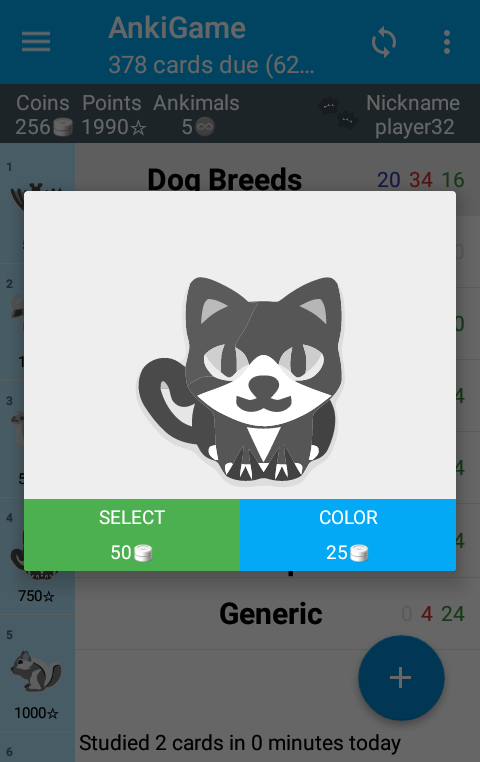
\includegraphics[scale=0.4]{./Figures/ankimal_selection.png}
            \caption{Dialog to select and color a rescued ankimal.}
            \label{fig:ankimals-select}
        \end{center}
    \vskip -5mm
\end{figure}

%----------------------------------------------------------------------------------------
\subsection{Social and Competition}
The informative nature of points was also used to integrate another common element of games: leaderboard. In the solution, the leadearboard had two objectives. First, it provided a social context to the users. Thus, they knew that there were other people using the application. The social context was boosted with the inclusion of nicknames and avatars as seen in Figure \ref{fig:leaderboard}. That meant users could have a broader context of their identities within the application. Not only were they able to define their nicknames and avatars, but the leadearboard also provided a way to see others'.

The second objective of the leadearboard was aimed at adding a new level of motivation for the revision of flashcards. Since positions in the leadearboard depended on the number of points, users needed to review more flashcards to increase the number of points, hence, improve their positions. In addition, the positions were depicted as chess pieces, which could be interpreted as achievements. However, unlike rescuing ankimals, reaching a position in the leadearboard was not definitive. A position in the leaderboard could be lost against other users.

\begin{figure}[htb]
    \vskip 5mm
        \begin{center}
            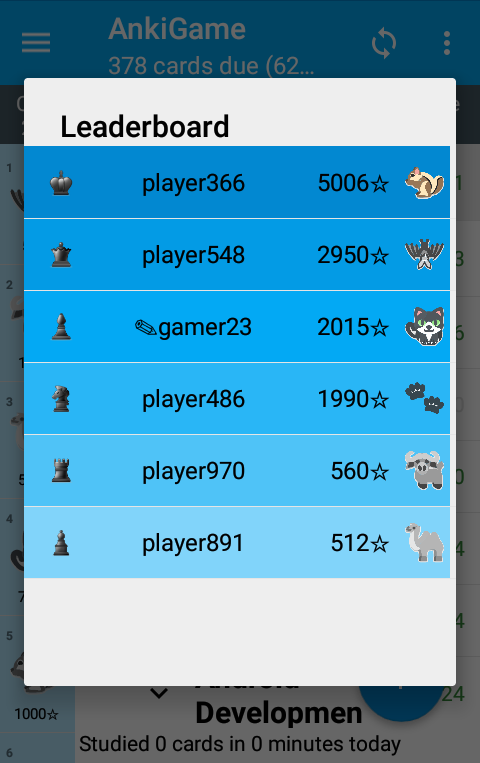
\includegraphics[scale=0.4]{./Figures/leaderboard.png}
            \caption{leadearboard showing the nicknames and avatars of users.}
            \label{fig:leaderboard}
        \end{center}
    \vskip -5mm
\end{figure}

%----------------------------------------------------------------------------------------
\subsection{Progress}
It was necessary to keep users informed about the state of the new gamification elements of the application. Similar to games that provide elements to inform about progress and other aspects, the solution added a status bar to provide information about the points, coins, rescued ankimals, avatar, and nickname. This new visual element was designed to be easily integrated into relevant parts of the application as seen in Figures \ref{fig:reviewer-modified} and \ref{fig:progress}, where it is located and constantly visible below the main bar of the application. Moreover, the design allowed instant updates of its elements.

\begin{figure}[htb]
    \vskip 5mm
        \begin{center}
            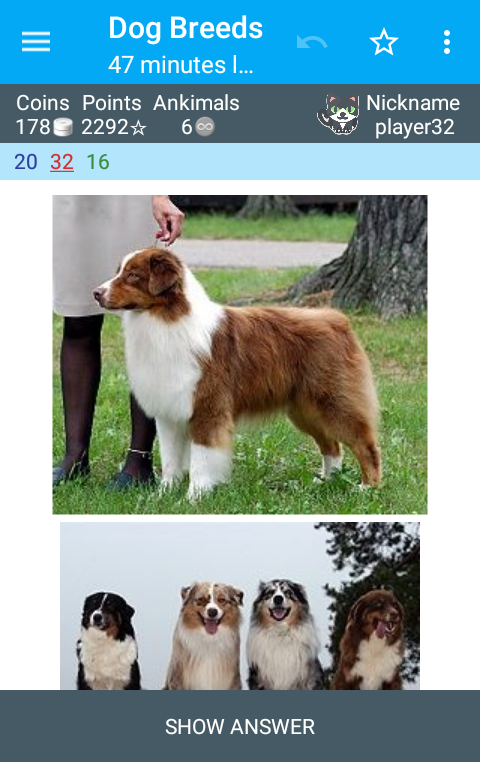
\includegraphics[scale=0.4]{./Figures/modified_reviewer.png}
            \caption{Modified flashcards reviewer displaying informative gamification elements.}
            \label{fig:reviewer-modified}
        \end{center}
    \vskip -5mm
\end{figure}

Additionally, a list of elements was also added in the deck picker to show the rescued and not rescued ankimals as seen in Figure \ref{fig:progress}. The list had the same informative purpose of the status bar; however, they differed in the interactions. While the status bar did not enable any kind of interactions, the list allowed users to pick any ankimal to set it as their avatar or add colour to it. The interactive nature of the list of ankimals was consistent with the list of pickable decks. Moreover, they shared the same vertical layout.

\begin{figure}[htb]
    \vskip 5mm
        \begin{center}
            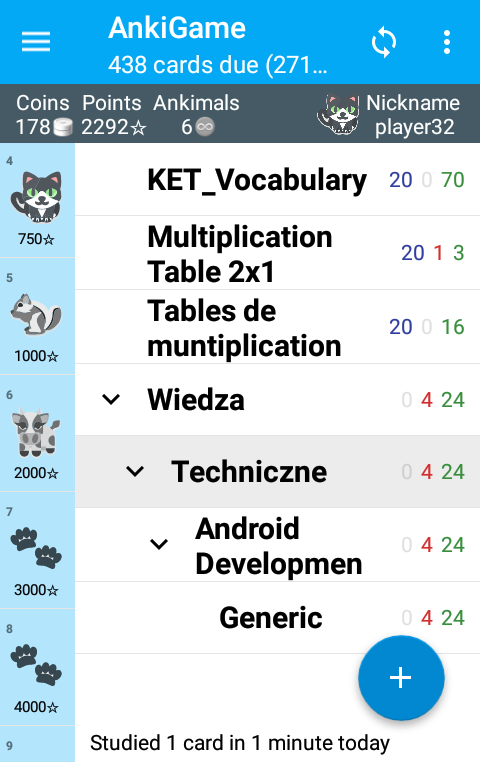
\includegraphics[scale=0.4]{./Figures/progress.png}
            \caption{Modified deck picker displaying informative gamification elements.}
            \label{fig:progress}
        \end{center}
    \vskip -5mm
\end{figure}

%----------------------------------------------------------------------------------------
\section{Game Integration}
\label{game-integration}
The most important design decision in the solution was the inclusion of a game. The integration of a game was the key difference with other gamification approaches. Unlike the previously described elements that added new features to existing functionalities, a game was a completely new component in the application. Therefore, it was required that the game be easy to play and avoided an unnecessary level of complexity. For this reason, a casual game was the most suitable option. Casual games are straightforward and their gameplays allow short periods of play, which convert them into activities that can be executed during work or study breaks.

The game needed to be integrated into AnkiDroid in a way that it fitted in the structure easily. Moreover, the integration required the definition of a linkage between the game and other components of the application. These conditions set the scenario to modify the game and use the previously described gamification elements. The final design set the game as a component with some flexibility to use and smoothly connected to the rest of the application. However, the design also included some constraints aimed at increasing the user engagement of flashcards revision.

%----------------------------------------------------------------------------------------
\subsection{Modifications to the Game}
2048 is a simple yet challenging game due to the high number of turns to form the block 2048 (1024 turns in the perfect case). Another aspect that increases the difficulty of the game is the limited space. If there are no more empty cells in the grid, and no further movements are possible, then the game is over. Such difficulty along with the need to connect the game with the rest of the application set the starting point to modify the game. Such modifications had to be consistent with the easy-to-use paradigm of casual games. Moreover, they needed to maintain a consistency such that their behaviour and results were easy to understand.

Based on the requirements to modify the game, a set of elements was defined to ease the gameplay. Those elements took the form of cheat tricks aimed at providing more alternatives to win. Each trick changed the state of the grid so that players had more options in a next move. The state of the grid was defined by the positions of the blocks and their values at a given turn. Therefore, there existed several approaches to change the state of the board. Moreover, each trick needed to provide a different degree of benefit; thus, they were not equally valuable. The modifications included four cheat tricks as seen in Table \ref{tab:tricks}. It is important to note the restrictions to use them based on the state of the grid.

\begin{table*}[!htb]
  \centering
  {\renewcommand{\arraystretch}{1}
    \begin{tabular}{|R{2cm}|R{6cm}|R{5cm}|}
    \hline
    \multicolumn{1}{|>{\centering\arraybackslash}m{2cm}|}{\textbf{Name}} &
    \multicolumn{1}{>{\centering\arraybackslash}m{6cm}|}{\textbf{Benefit}} &
    \multicolumn{1}{>{\centering\arraybackslash}m{5cm}|}{\textbf{Usage conditions}}\\
    \hline
    Gift & Adds a randomly positioned block that can merge with any block whose value is less than 512. & There is at least one empty cell in the grid.\\
    \hline
    Doubler & Doubles all the blocks whose values are 2. & There is at least one block with a value of 2 in the grid.\\
    \hline
    Remover & Removes all the blocks whose values are 2. & There is at least one block with a value of 2 in the grid. \newline There is least one block with a value greater than 2.\\
    \hline
    Undo & Undoes the last movements (up to 10 previous movements). & There are previous movements.\\
    \hline
    \end{tabular}
  }
  \caption{Cheat tricks for the game, their benefits, and usage conditions.}
  \label{tab:tricks}
\end{table*}

%----------------------------------------------------------------------------------------
\subsection{Connection with Flashcards Revision}
A connection meant finding existing elements in AnkiDroid that could act as the glue material between the game and the revision of flashcards. In other words, the connection had to be done to include a motivational aspect to encourage users to review more flashcards to obtain benefits in the game. Thus, the user engagement could increase by adopting elements from AnkiDroid to the logic and structure of the game. The original application did not present elements that could be easily adjusted to the game. However, two of the gamification elements defined earlier provided a way to make the connection.

The first elements were points, which already provided a motivational aspect in the revision of flashcards. The informative nature of points was previously used to define achievements in the revision of flashcards. Following the same scheme, they were also used to define achievements in the game. In this case, the cheat tricks in the game were linked to a specific number of points based on the benefits they provided; the higher the benefit, the higher the number of points. Therefore, the tricks were initially hidden, then, users needed to obtain the corresponding number of points to reveal each trick. Finally, unlike ankimals, users were not notified when a trick was revealed since the main interest was the revision of flashcards, not playing the game.

The number of available tricks was small (4), and revealing each of them was a one-time event. This situation could potentially limit the connection between the game and the revision of flashcards. Therefore, it was necessary to take advantage of coins, which were already used as resources to select and colour ankimals. In the game, once the tricks were revealed, players could use them at any point as long as they had the required number of coins. In some sense, users needed to buy tricks with the coins they earned reviewing flashcards. Similarly, a specific number of coins was set for each trick based on the benefit level as seen in Table \ref{tab:tricks-coins-points}.

\begin{table*}[!htb]
  \centering
  {\renewcommand{\arraystretch}{1}
    \begin{tabular}{|R{3cm}|R{3cm}|R{2cm}|R{2cm}|}
    \hline
    \multicolumn{1}{|>{\centering\arraybackslash}m{3cm}|}{\textbf{Cheat trick}} &
    \multicolumn{1}{>{\centering\arraybackslash}m{3cm}|}{\textbf{Benefit level}} &
    \multicolumn{1}{>{\centering\arraybackslash}m{2cm}|}{\textbf{Points}} &
    \multicolumn{1}{>{\centering\arraybackslash}m{2cm}|}{\textbf{Coins}}\\
    \hline
    Gift & Low & 100 & 10\\
    \hline
    Doubler & Medium & 500 & 20\\
    \hline
    Remover & High & 1000 & 30\\
    \hline
    Undo & Higher & 2000 & 40\\
    \hline
    \end{tabular}
  }
  \caption{Costs of cheat tricks in terms of points to reveal and coins to use them.}
  \label{tab:tricks-coins-points}
\end{table*}

%----------------------------------------------------------------------------------------
\section{User Interface Considerations}
Several user interface aspects were considered to implement the game elements described earlier. First, the modifications in the game required the addition of interactive elements for each cheat trick. Initially, colour information was used to differentiate the cheat tricks and to provide clues about their status (blocked, enabled, usable)  as seen in Figure \ref{fig:modified-game}. Moreover, since the gameplay required the users to slide vertically and horizontally, cheat tricks could easily be selected by mistake. Avoiding that problem required designing a translucent curtain to be removed by the user before selecting cheat tricks.

\begin{figure}[htb]
    \vskip 5mm
        \begin{center}
            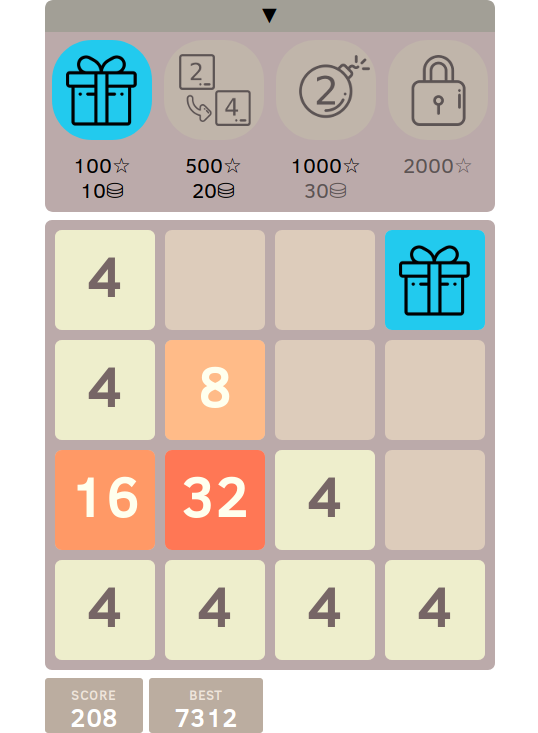
\includegraphics[scale=0.4]{./Figures/modified_game.png}
            \caption{Modified game showing the cheat tricks with different status at the top of the grid.}
            \label{fig:modified-game}
        \end{center}
    \vskip -5mm
\end{figure}

In AnkiDroid, the main considerations to implement the game elements were related to keeping consistency in the overall aspect of the application and the visual clues for the user. The first aspect required using the same colour scheme along with other elements like the font type and size. On the other hand, visual clues were meant to provide information about modifications in the game elements. This was done by implementing animations where necessary. For instance, when the number of coins or points changed, animations that updated the corresponding visual elements were implemented. Finally, the visual structure was maintained as much as possible to avoid the new components from being intrusive.

%  % Use this as criticism
%  Evidently, users could play the game without using tricks, but






 
%% Chapter 5

\chapter{Experimental setup} % Main chapter title

\label{expe} % For referencing the chapter elsewhere, use \ref{Chapter5}

\lhead{Chapter 5. \emph{Experimental setup}} % This is for the header on each page - perhaps a shortened title

The proposed solution was tested in an study that required the definition of several conditions. First, it required to define the types of data to be collected. Then, the structure of data and the mechanisms of collection were established. It was also important to identify the type of participants and divide them groups to test different versions of the application. The versions of the application were distributed over a platform to let participants install them with ease. Finally, the study was set over a period of time, and the application was delivered to a broader audience.

%----------------------------------------------------------------------------------------
\section{Data}
The required data to analyse and evaluate the solution came from two sources. The first source was the application itself, here the data was automatically generated from the users' interactions. This type of data had a quantitative nature, therefore, it was possible to measure and analyse it from a statistical point of view. The second source of information was users who provided feedback about their experience in the form of comments and suggestions. This type of data had a qualitative nature, thus the analysis was different and required other type of tools.

Quantitative and qualitative data gave different perspectives about the use of the application. However, they were not necessarily mutually exclusive, a careful analysis complemented each other and gave more insights about the overall user experience. Another key difference between both types of data was the period of collection. Quantitative data were collected from the start to the end of the period of the study, whereas qualitative data were collected at the end. Finally, qualitative were obtained from the participants only, whereas quantitative data came from the participants and a broader audience.

Originally, AnkiDroid collects a lot of usage information which is available to users in the form of statistics. These data are quantitative and give users a perspective about their progress based on the number of flashcards review, the number of sessions, the amount of time in sessions and more. The application even forecasts the number of flashcard to be reviewed in the near future. This information was not collected for analysis since it provides a general overiew of the usage from the perspective of users, and lacks details related to the integrated game and the gamification elements

\section{Collection and structure of data}
Quantitative data were generated in points where users interacted with the application e.g. playing the game, selecting a deck, or reviewing flashcards. Each time an important interaction was done, the application processed the relevant information and sent it to an external server to persist it. Therefore, it was necessary to define an scheme to format the information before store it. The format was also aimed to facilitate the analysis and interpretation of results. Thus, quantitative information was grouped in four categories as seen in Table \ref{tab:info-type}.

\begin{table*}[!htb]
	\centering
	{\renewcommand{\arraystretch}{2}
		\begin{tabular}{|R{3cm}|R{6cm}|}
		\hline
		\multicolumn{1}{|>{\centering\arraybackslash}m{2cm}|}{\textbf{Category}} &
		\multicolumn{1}{>{\centering\arraybackslash}m{6cm}|}{\textbf{Description}} \\
		\hline
		Common & Details of time and user.\\
		\hline
		Game & Details about the game.\\
		\hline
		Gamification & Details of game elements. \\
		\hline
		Anki & Details of flashcards and decks. \\
		\hline
		\end{tabular}
	}
	\caption{Categories of quantitative information collected from the application.}
	\label{tab:info-type}
\end{table*}

The common category was meant to identify the time, date and user that generate the interaction. This type of data was part of every relevant interaction in the application. The next category of information was related to the game; it included details about the score, cheat tricks, and state of the grid. The gamification category had to do with the added game elements to AnkiDroid, it included details about the number of coins, number of points, and names of the ankimals. Finally, the anki category refered to details about the decks, flashcards, and revision times.

The categories of information were stored in the form of logs. Logs were an scheme to assemble and structure information from different categories based on the relevant interactions generated in the application. Logs were grouped in two main classes: game logs and anki logs. Games logs contained information from the game category, however, some data from the gamification category was also registered in these logs. Anki logs contained information from Anki category with some data from the gamification category. Information of common category was recorded in both groups of logs as seen in Figure \ref{fig:categories-logs}.

\begin{figure}[htb]
    \vskip 5mm
        \begin{center}
            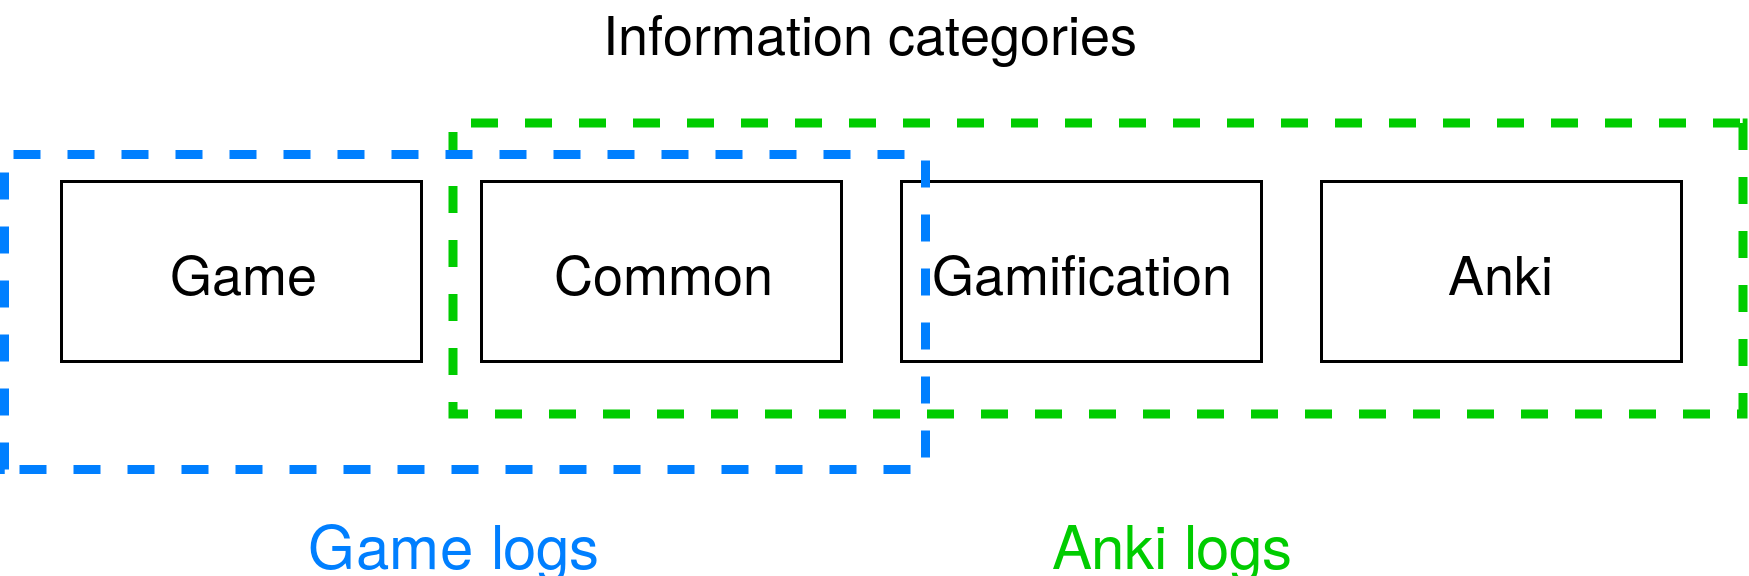
\includegraphics[scale=0.7]{./Figures/categories_logs.png}
            \caption{Types of logs and their relation to information categories.}
            \label{fig:categories-logs}
        \end{center}
    \vskip -5mm
\end{figure}

Specifically speaking there were 6 types of game logs and 9 types of anki logs as shown in Table \ref{tab:log-types}. Game logs were generated in the game context. Something similar occured with anki logs, however, the design of the solution allowed one anki log to be generated in the game context: Check leaderboard. This was possible because users could open the leader-board either in the game context or in the anki context. The reason for this design is that the leaderboard provides information of social aspect. Despite the fact that the leader-board display gamification data (points), users were not asked to do an specific action in anki or the game contexts to see their positions.

\begin{table*}[!htb]
	\centering
	{\renewcommand{\arraystretch}{2}
		\begin{tabular}{ |c|c|c| }
			\hline
			\textbf{Type of log} & \textbf{Name of log} \\
			\hline
			\multirow{6}{3cm}{Game log} &  Game won\\
			& Game lost \\
			& Game restarted \\
			& Trick used \\
			& Trick failed \\
			& Switched to anki \\
			\hline
			\multirow{9}{3cm}{Anki log} &  Leaderboard checked\\
			& Custom study set \\
			& Flashcard answer revealed\\
			& Flashcard assessed \\
			& Deck selected \\
			& Ankimal rescued\\
			& Ankimal selected\\
			& Ankimal colored\\
			& Switched to game \\
			\hline
		\end{tabular}
	}
	\caption{Types of logs collected from the application.}
	\label{tab:log-types}
\end{table*}

Collecting qualitative data required the direct participation of the users to complete a survey. The survey had a set of questions aimed to gather information about the perception of the participants about the application. The majority of the questions required the user to select one or more options, however, the participants were also provide additional comments or suggestions. Even though, the survey was the main source of qualitative data, additional comments and suggestions about the application were given by participants and other people via email or comments in the forums and communities where the application was advertised for the general public.


%----------------------------------------------------------------------------------------
\section{Participants}
\label{participants}
The study required to recruit a group of participants to use the application. The main requirement was to have an Android device to install the application. It was not necessary that participants had an especific profile. However, to mantain some level of homogeneity, the recruitment was done based on previous experience with AnkiDroid or other interfaces of Anki. The selected participants did not have any previous contact with Anki. Therefore, they were new to this educational tool and the modifications explained in chapter \ref{desi}.

Participants were recruited while the application was in the development phase. During this process they were informed about the objective and duration of the study. Since, they did not have any previous experience with AnkiDroid, they were taught about the objective, benefits, and functionalities of the application. In addition, they were also instructed about the gamification features and the casual game. Participants were not forced to be part of the study from start to end. They were free to live the study at any point as this situation provided additional insights about the application.

%----------------------------------------------------------------------------------------
\section{Groups of participants}
As described in section \ref{game-integration}, the key difference between the proposed solution and others was the the inclusion of a casual game. For this reason, the application was split in two versions. The first version had the causal game and all the other gamification elements; this version was named AnkiGame. The second version did not have the integrated game, but the other gamification elements were available; this version was named AnkiPlay. Therefore, it was possible to analyse the effectiveness of the integration of a casual game as a means to increase user engagement.

The two versions of the application caused that the participants were randomly separated in two sets with six members in each one. The resulting sets were defined as the control group and the experimental group. Participants in the control group were given the AnkiPlay version, whereas participants in the second group were given the AnkiGame version as seen in Figure \ref{fig:participants-version}. None of the participants were told about the existence of the other version of the application. This decision was made to reduce any potential bias in the use of the application.

\begin{figure}[htb]
    \vskip 5mm
        \begin{center}
            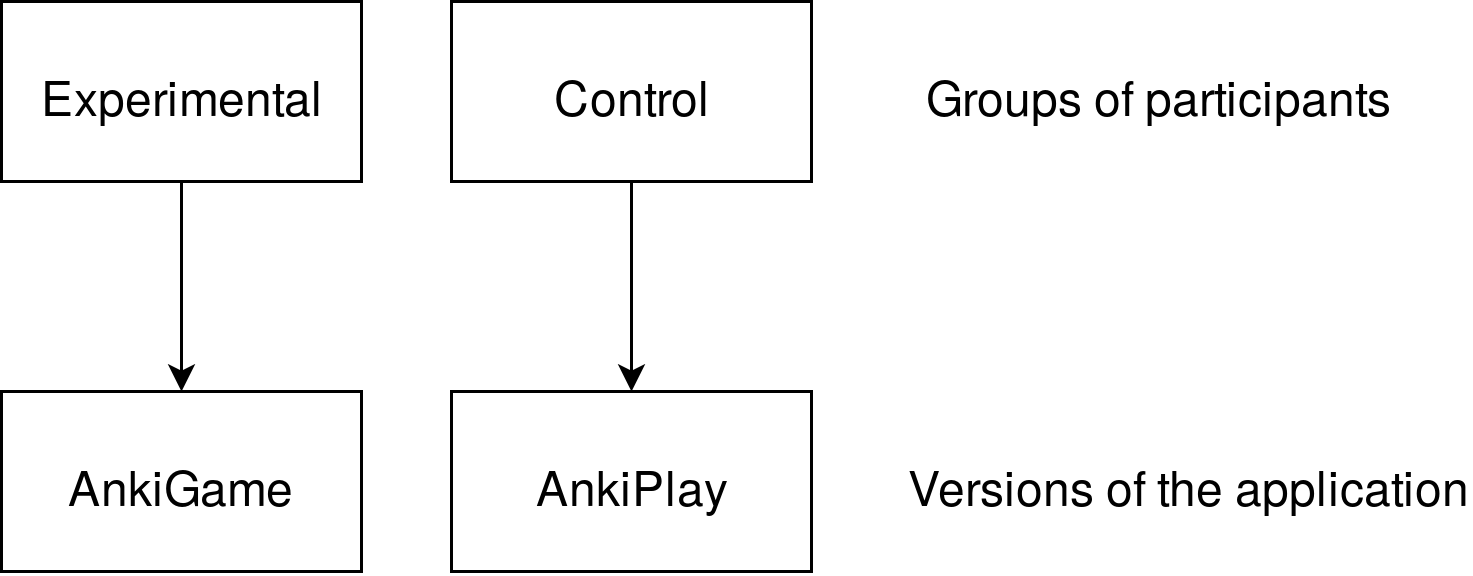
\includegraphics[scale=0.7]{./Figures/participants_version.png}
            \caption{Gropus of participants and the assigned versions of the application.}
            \label{fig:participants-version}
        \end{center}
    \vskip -5mm
\end{figure}

%----------------------------------------------------------------------------------------
\section{Distribution of the application}
The application was distributed in the Google Play Store. This platform allows to have multiple versions of the same application in independent contexts. Therefore, it was possible to publish AnkiGame and AnkiPlay simultaneously. Thus, participants had an easy way to find and install the correspoding version in their devices. Another advantage of this platform is the different testing stages it offers. This feature was used to set a beta testing phase where potential issues were found and additional improvements were added to the application before making it available to participants.

In addition, Google Play Store allows making updates to correct bugs, add new features, or release new versions of an application. The updates are automatically installed in devices that already have the corresponding applications. Moreover the distribution platform provides insights about use and performance in the form of statistics. Users have the option to provide additional quantitative data by rating the application. Qualitative data is also available in the form of comments and suggestions left in the page of each application.

%----------------------------------------------------------------------------------------
\section{Duration of study and broader audience}
The study was set to last four weeks when participants used the application and generated data. The study period was divide in two stages as seen in \ref{fig:study-period}. The first stage lasted three weeks and users were suggested to use the application at least during this period, but as explained in section \ref{participants}, they were not forced to do so. At the end of this period, participants could stop using the application. For the second stage, participants were recommended to keep using the application if they wanted to. At the end, participants were asked to complete a survey. An study with two phases was intended to provide more insights about the use of the application from those participants kept using it.

\begin{figure}[htb]
    \vskip 5mm
        \begin{center}
            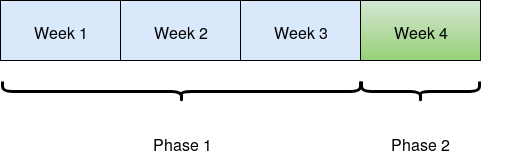
\includegraphics[scale=0.7]{./Figures/study_period.png}
            \caption{Duration and phases of the study period.}
            \label{fig:study-period}
        \end{center}
    \vskip -5mm
\end{figure}

Since the application was openly distributed in Google Play Store, it was possible to make it available to a broader audience. Therefore, additional data were gotten from other people. This data provided extra insights about the use of the application. In this case, the application was advertised in AnkiDroid forums, therefore, it is likely the majority of new users had a previous contact with the original application. Therefore, the information from these new users were isolated from the information from the participants to avoid any incorrect analysis. The users that were not part of the original study were also informed about the nature and objectives of the application.
 
%% Chapter 5

\chapter{Evaluation and Results} % Main chapter title

\label{resu} % For referencing the chapter elsewhere, use \ref{Chapter1}

% \lhead{Chapter 6. \emph{Evaluation and Results}} % This is for the header on each page - perhaps a shortened title
The data collected from the study was processed and compiled to extract information aimed at evaluating the effectiveness of the integration of a casual game as part of the gamification strategy. The evaluation was done in terms of user engagement, which required the definition of some metrics. These metrics provided insights into the behaviour of users in every group. Then, a hypothesis testing showed that the user engagement did not present a statistically significant variation between the control and experimental groups.

%----------------------------------------------------------------------------------------
\section{User Engagement Metrics}
Evaluating the solution in terms of user engagement required the definition of some metrics. There are many alternatives to measure user engagement in mobile applications. The selection of one option over others depends on the aim of every application. As seen in Section \ref{desi-components-interest}, the core element of AnkiDroid is the flashcard reviewer. This component is where users get the benefits from the effects of spaced repetition. Therefore, the metrics of use for user engagement are defined around the actions and parameters that depended on the interactions done in this element.

Based on the original functionality of the flashcard reviewer, the first metric was the total number of flashcards reviewed during the period of study. This metric included the repetitions of flashcards since they are the foundations of the spaced repetition technique. Thus, the metric did not consider the performance of users. In other words, it did not penalise users based on their previous knowledge or ability to learn new things.

The flashcard reviewed was modified to include the earning of coins and points. These two parameters were also considered for the evaluation since they gave additional information about the number of flashcards. It is important to note that, as expressed in Equations \ref{eq:coins-formula} and \ref{eq:points-formula}, the number of points and coins depended on the time reviewing flashcards, which complemented the information from the total number of cards.

The total number of flashcards reviewed by each user depends on the amount of content of every flashcard. Since users were free to review flashcards based on their interests, chances are that they did not use the same decks. Therefore, the number of flashcards might not provide enough information. For this reason, another metric of use was the amount of time (measured in seconds) reviewing flashcards. This information was somehow encapsulated in the number of coins and points, but as seen in Equations \ref{eq:coins-formula} and \ref{eq:points-formula}, some flashcards could have given zero points and coins.

Other important metrics obtained from the compiled logs included the number of interactions, days using the application, average interactions per day (AIPD), the period of use, average time between sessions (ATBS), and the number of decks. The values of these metrics are detailed in Tables \ref{tab:summ_control} and \ref{tab:summ_experimental}. At a glance, the values are better for the experimental group, e.g., the number of reviewed flashcards is visually higher for the experimental group as seen in Figures \ref{fig:cards-control} and \ref{fig:cards-experimental}. However, these comparisons are not enough to evaluate the user engagement.

\begin{table*}[!htb]
    \centering
    \small
    \vspace{1cm}
    {\renewcommand{\arraystretch}{1}
        \begin{tabular}{|R{4.5cm}|R{1cm}|R{1cm}|R{1cm}|R{1cm}|R{1cm}|R{1cm}|}
        \hline
        \multicolumn{1}{|>{\arraybackslash}m{4.5cm}|}{\textbf{Participant}} &
        \multicolumn{1}{>{\centering\arraybackslash}m{1cm}|}{1} &
        \multicolumn{1}{>{\centering\arraybackslash}m{1cm}|}{2} &
        \multicolumn{1}{>{\centering\arraybackslash}m{1cm}|}{3} &
        \multicolumn{1}{>{\centering\arraybackslash}m{1cm}|}{4} &
        \multicolumn{1}{>{\centering\arraybackslash}m{1cm}|}{5} &
        \multicolumn{1}{>{\centering\arraybackslash}m{1cm}|}{6} \\
        \hline
        \textbf{Total cards} & 738 & 125 & 51 & 40 & 37 & 0 \\ \hline
        \textbf{Total points} & 1990 & 263 & 402 & 131 & 252 & 0 \\ \hline
        \textbf{Total coins} & 818 & 93 & 173 & 54 & 105 & 0 \\ \hline
        \textbf{Time in cards (seconds)} & 2317 & 386 & 354 & 143 & 223 & 0 \\ \hline
        \textbf{Interactions} & 1532 & 266 & 106 & 88 & 83 & 2 \\ \hline
        \textbf{Days using app} & 12 & 5 & 2 & 2 & 3 & 1 \\ \hline
        \textbf{Period of use (days)} & 22 & 11 & 8 & 2 & 8 & 1 \\ \hline
        \textbf{Decks} & 3 & 3 & 3 & 3 & 2 & 1 \\ \hline
        \textbf{AIPD} & 128 & 53 & 53 & 44 & 28 & 2 \\ \hline
        \textbf{ATBS (days)} & 1.8 & 2.2 & 4 & 1 & 2.6 & 1 \\ \hline
        \end{tabular}
    }
    \caption{User engagement metrics per user in control group.}
    \label{tab:summ_control}
\end{table*}

\begin{table*}[!htb]
    \centering
    \small
    \vspace{1cm}
    {\renewcommand{\arraystretch}{1}
        \begin{tabular}{|R{4.5cm}|R{1cm}|R{1cm}|R{1cm}|R{1cm}|R{1cm}|R{1cm}|}
        \hline
        \multicolumn{1}{|>{\arraybackslash}m{4.5cm}|}{\textbf{Participant}} &
        \multicolumn{1}{>{\centering\arraybackslash}m{1cm}|}{1} &
        \multicolumn{1}{>{\centering\arraybackslash}m{1cm}|}{2} &
        \multicolumn{1}{>{\centering\arraybackslash}m{1cm}|}{3} &
        \multicolumn{1}{>{\centering\arraybackslash}m{1cm}|}{4} &
        \multicolumn{1}{>{\centering\arraybackslash}m{1cm}|}{5} &
        \multicolumn{1}{>{\centering\arraybackslash}m{1cm}|}{6} \\
        \hline
        \textbf{Total cards} & 745 & 625 & 370 & 114 & 74 & 51\\ \hline
        \textbf{Total points} & 6221 & 1152 & 1311 & 1489 & 447 & 211\\ \hline
        \textbf{Total coins} & 2169 & 449 & 549 & 460 & 163 & 78\\ \hline
        \textbf{Time in cards (seconds)} & 7826 & 1495 & 1252 & 2433 & 554 & 252\\ \hline
        \textbf{Interactions} & 1699 & 1301 & 1250 & 294 & 180 & 114\\ \hline
        \textbf{Days using app} & 12 & 9 & 28 & 6 & 7 & 3\\ \hline
        \textbf{Period of use (days)} & 18 & 14 & 28 & 12 & 22 & 3\\ \hline
        \textbf{Decks} & 16 & 4 & 4 & 5 & 3 & 2\\ \hline
        \textbf{AIPD} & 142 & 145 & 45 & 49 & 26 & 38\\ \hline
        \textbf{ATBS (days)} & 1.5 & 1.5 & 1 & 2 & 3.1 & 1\\ \hline
        \end{tabular}
    }
    \caption{User engagement metrics per user in experimental group.}
    \label{tab:summ_experimental}
\end{table*}

\begin{figure}[htb]
    \vskip 5mm
        \begin{center}
            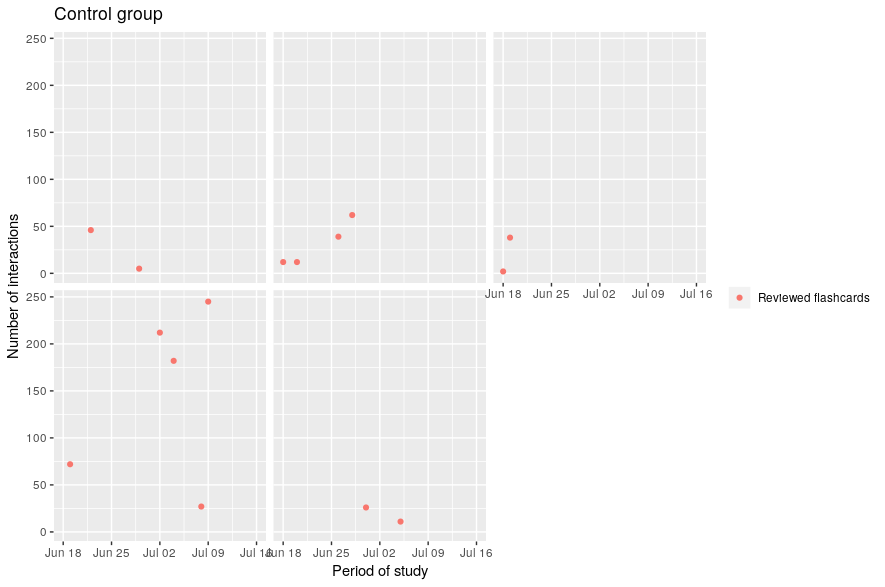
\includegraphics[scale=0.75]{./Figures/con_n_flashcards.png}
            \caption{Number of reviewed flashcards per user in the control group.}
            \label{fig:cards-control}
        \end{center}
    \vskip -5mm
\end{figure}

\begin{figure}[htb]
    \vskip 5mm
        \begin{center}
            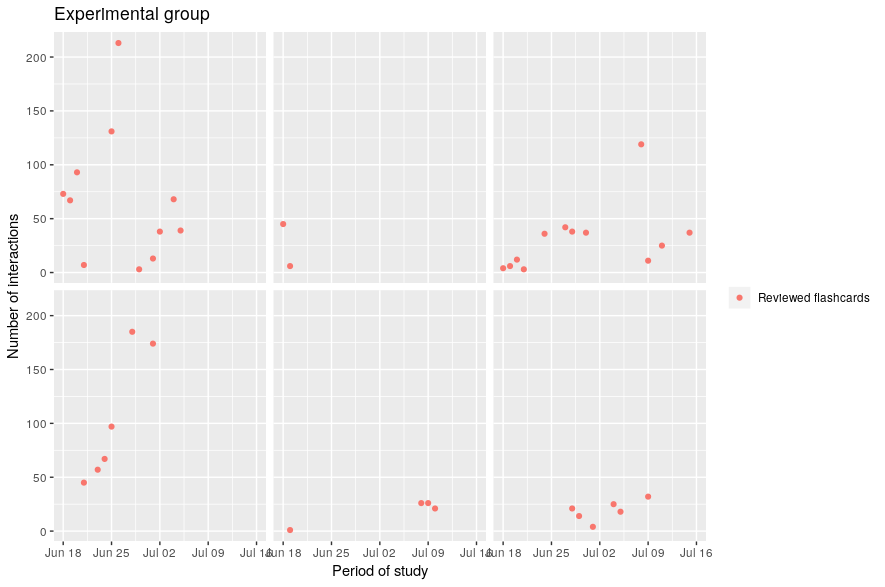
\includegraphics[scale=0.75]{./Figures/exp_n_flashcards.png}
            \caption{Number of reviewed flashcards per user in the experimental group.}
            \label{fig:cards-experimental}
        \end{center}
    \vskip -5mm
\end{figure}

%----------------------------------------------------------------------------------------
\section{Hypothesis Testing}
The proposed solution was designed to implement a gamification strategy that integrated a casual game. The objective was to provide users another extrinsic motivational element aimed at increasing user engagement. In other words, the goal of the project was the integration of a casual game as part of the gamification strategy to increase user engagement. Specifically, the hypothesis for the study was formulated as follows:

\begin{displayquote}
\textbf{User engagement is higher in the experimental group than in the control group.}
\end{displayquote}

The hypothesis was tested using the Student's t-test analysis over the defined user engagement metrics. This required defining the null hypothesis as follows:

\begin{displayquote}
\textbf{User engagement does not differ in the experimental group and the control groups.}
\end{displayquote}

The results of the t-test are shown in Table \ref{tab:t_test}. As can be seen, the majority of mean absolute values are larger in the experimental group. However, the p-values are not significantly small, which means that the null hypothesis could not be rejected. Moreover, the intervals of confidence at 95\% confirm that the results are not statistically significant, as seen in Figure \ref{fig:metrics}. Therefore, the difference of the means for every metric were due to chance. Thus, it was not possible to conclude that user engagement was affected by the integration of a casual game in a gamification strategy. Similar results were obtained from the data collected from users of a broader audience as seen in Table \ref{tab:t_test_broader}.


\begin{table*}[!htb]
    \centering
    \small
    \vspace{1cm}
    {\renewcommand{\arraystretch}{1}
        \begin{tabular}{|R{4.5cm}|R{1.5cm}|R{1.5cm}|R{1cm}|R{1cm}|}
        \hline
        \multicolumn{1}{|>{\arraybackslash}m{4.5cm}|}{\textbf{Metric}} &
        \multicolumn{1}{>{\centering\arraybackslash}m{2cm}|}{$\mu$ CG} &
        \multicolumn{1}{>{\centering\arraybackslash}m{2cm}|}{$\mu$ EG} &
        \multicolumn{1}{>{\centering\arraybackslash}m{2cm}|}{t-value} &
        \multicolumn{1}{>{\centering\arraybackslash}m{2cm}|}{p-value} \\
        \hline
        \textbf{Total cards} & 65.2 & 329.8 & -0.98 & 0.35\\ \hline
        \textbf{Total points} & 506.3 & 1805.2 & -1.36 & 0.22\\ \hline
        \textbf{Total coins} & 207.2 & 644.7 & -1.29 & 0.24\\ \hline
        \textbf{Time in cards (seconds)} & 570.5 & 2302 & -1.44 & 0.20\\ \hline
        \textbf{Interactions} & 346.2 & 806.3 & -1.25 & 0.24\\ \hline
        \textbf{Days using app} & 4.2 & 10.8 & -1.66 & 0.14\\ \hline
        \textbf{Period of use (days)} & 8.7 & 16.2 & -1.60 & 0.14\\ \hline
        \textbf{Decks} & 2.5 & 5.7 & -1.48 & 0.20\\ \hline
        \textbf{AIPD} & 51.3 & 74.2 & -0.81 & 0.43\\ \hline
        \textbf{ATBD (days)} & 2.1 & 1.7 & 0.74 & 0.48\\ \hline
        \end{tabular}
    }
    \caption[T-test values for user engagement metrics in the study groups.]{T-test values for user engagement metrics in the study groups. CG stands for control group, EG stands for experimental group.}
    \label{tab:t_test}
\end{table*}

\begin{table*}[!htb]
    \centering
    \small
    \vspace{1cm}
    {\renewcommand{\arraystretch}{1}
        \begin{tabular}{|R{4.5cm}|R{1.5cm}|R{1.5cm}|R{1cm}|R{1cm}|}
        \hline
        \multicolumn{1}{|>{\arraybackslash}m{4.5cm}|}{\textbf{Metric}} &
        \multicolumn{1}{>{\centering\arraybackslash}m{2cm}|}{$\mu$ AP} &
        \multicolumn{1}{>{\centering\arraybackslash}m{2cm}|}{$\mu$ AG} &
        \multicolumn{1}{>{\centering\arraybackslash}m{2cm}|}{t-value} &
        \multicolumn{1}{>{\centering\arraybackslash}m{2cm}|}{p-value} \\
        \hline
        \textbf{Total cards} & 1815.42 & 524.67 & 0.74 & 0.48\\ \hline
        \textbf{Total points} & 14156.33 & 5087.10 & 0.58 & 0.57\\ \hline
        \textbf{Total coins} & 5106.25 & 1676.92 & 0.68 & 0.50\\ \hline
        \textbf{Time in cards (seconds)} & 15493.33 & 10400.92 & 0.30 & 0.77\\ \hline
        \textbf{Interactions} & 3707 & 1126.5 & 0.72 & 0.49\\ \hline
        \textbf{Days using app} & 5.33 & 5.83 & -0.13 & 0.90\\ \hline
        \textbf{Period of use (days)} & 8.58 & 6.50 & 0.48 & 0.63\\ \hline
        \textbf{Decks} & 3.75 & 3.5 & 0.14 & 0.89\\ \hline
        \textbf{AIPD} & 178.5 & 50.25 & 0.91 & 0.38\\ \hline
        \textbf{ATBS (days)} & 1.90 & 1.08 & 1.83 & 0.09\\ \hline
        \end{tabular}
    }
    \caption[T-test values for user engagement metrics in the broader audience.]{T-test values for user engagement metrics in the broader audience. AP stands for AnkiPlay, AG stands for AnkiGame.}
    \label{tab:t_test_broader}
\end{table*}

\begin{figure}[htb]
    \vskip 5mm
        \begin{center}
            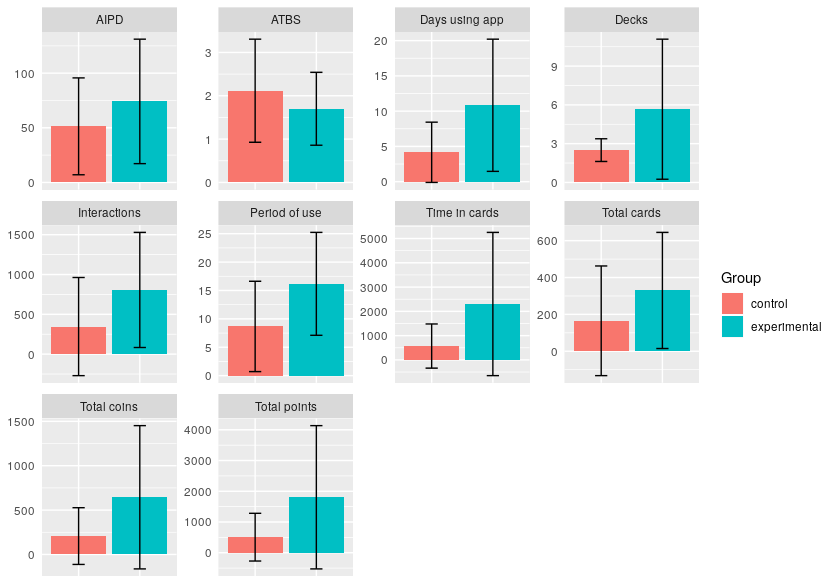
\includegraphics[scale=0.75]{./Figures/metrics.png}
            \caption{Means and intervals of confidence at 95\% for every metric.}
            \label{fig:metrics}
        \end{center}
    \vskip -5mm
\end{figure} 
%% Chapter 6

\chapter{Conclusions} % Main chapter title

\label{conc} % For referencing the chapter elsewhere, use \ref{Chapter1}

\lhead{Chapter 7. \emph{Conclusions}} % This is for the header on each page - perhaps a shortened title

The present work described the process to gamify an educational tool along with an evaluation based on the results obtained from data collected from new users of the application. The discussion was based around potential issues in the designed gamification strategy as well as the profile of the selected participants. It is important to note that gamification and other techniques that include extrinsic motivational elements are unlikely to give good results if the users lack the intrinsic motivation. Finally, a set of future projects were proposed based on the results and potential issues of the presented solution.

%----------------------------------------------------------------------------------------
\section{Discussion}
Gamification provides a way to include extrinsic motivational elements in different contexts. In educational tools, these elements can be used to make the learning experience more appealing which might be reflected in a higher user engagement. The current project presented a gamification strategy in AnkiDroid aimed at increasing user engagement. The key difference with other gamification alternatives was the integration of a casual game as an additional motivational element. The results showed that the proposed alternative did not have a statistical significance variation of user engagement compared to a traditional gamification strategy.

The structure of the solution was aimed at creating a link between the revision of flashcards and the casual game such that users had an extrinsic motivation to review more flashcards. However, one of the potential issues of the solutions might have been the flow of the connection between the game and the flashcards revision. Switching between the game and the revision of flashcards used the deck picker as an intermediary point. The design was done in that way considering that the deck picker was the place in the application to get access to other functionalities.

Since the participants selected for the study did not have previous experience using AnkiDroid, the learning curve to use the application might have been another potential issue. AnkiDroid is a mature application, but it contains many features that might be difficult to understand at the beginning. Moreover, the application presents information to users that makes sense as long as they understand some concepts of spaced repetition. In addition, the modifications done to the application added an extra complexity to the application even though they were implemented to not be intrusive.

In addition, it is important to note that gamification provides the tools to include additional extrinsic motivational elements. It is critical that the users have the intrinsic motivation i.e. learning something. If users are not interested in getting the benefits of an educational tool, other extrinsic motivational elements are unlikely to help. In the study, the participants might have lacked the intrinsic motivations, hence, they might have been lacking interest in the application overall.

%----------------------------------------------------------------------------------------
\section{Future work}
The presented work used a gamification strategy that integrated a casual game aimed at increasing user engagement in AnkiDroid. The obtained results were non-conclusive about the gamification strategy and further evaluation must be performed. However, this does not mean that gamification has to be discarded as an alternative to improve the user experience. Based on the potential issues discussed before, additional work can be done aimed at testing the effectiveness of the gamification strategy with people that are guaranteed to have the intrinsic motivation e.g. students of different educational levels, employees starting a new job, or people interested in learning new topics from a specific field.

Gamification techniques can also be studied in the context of facilitating the use of tools to new users. As discussed, AnkiDroid has an important level of complexity that requires users to spend some time to understand its features and functionalities. A gamification strategy could be aimed at providing a better user experience for new users and increase the retention. Moreover, the effects of gamification can also be studied in more advanced users only. 

%----------------------------------------------------------------------------------------
%	THESIS CONTENT - APPENDICES
%----------------------------------------------------------------------------------------

\addtocontents{toc}{\vspace{2em}} % Add a gap in the Contents, for aesthetics

\appendix % Cue to tell LaTeX that the following 'chapters' are Appendices

% Include the appendices of the thesis as separate files from the Appendices folder
% Uncomment the lines as you write the Appendices

% Appendix A

\chapter{Appendix Title Here} % Main appendix title

\label{AppendixA} % For referencing this appendix elsewhere, use \ref{AppendixA}

\lhead{Appendix A. \emph{Appendix Title Here}} % This is for the header on each page - perhaps a shortened title

Write your Appendix content here.
%\input{Appendices/AppendixB}
%\input{Appendices/AppendixC}

\addtocontents{toc}{\vspace{2em}} % Add a gap in the Contents, for aesthetics

\backmatter

%----------------------------------------------------------------------------------------
%	BIBLIOGRAPHY
%----------------------------------------------------------------------------------------

\label{Bibliography}

\lhead{\emph{Bibliography}} % Change the page header to say "Bibliography"

\bibliographystyle{apalike} % Use the "apalike" BibTeX style for formatting the Bibliography

\bibliography{Bibliography} % The references (bibliography) information are stored in the file named "Bibliography.bib"

\end{document}